%% The CSAIL abstract book is a custom document class called 
%% "csailabstractbook".  It is based on the teTeX 1.0 distribution of LaTeX,
%% insofar as it uses a number of additional packages from teTeX for its
%% behind-the-scenes formatting. If you are using a different
%% distribution of LaTeX, it is possible that your distribution does not
%% have the necessary packages, in which case you will receive a missing 
%% package error when using the class file. You may wish to latex a copy 
%% of this file as-is to ensure that your configuration is correct.  

%% You should *not* include additional packages in preparing your
%% abstract.  The csailabstractbook class automatically includes the
%% standard "graphicx" package for inclusion of figures. An example of
%% its syntax is given in the text below, and more detailed documentation
%% can be found from the lab's latex page. Please use PDF files for your images.

%% Producing your abstract should be straightforward. Keeping all your
%% files in your working directory, run latex on the abstract file, bibtex
%% on the abstract file, and then latex on the abstract file twice.

\documentclass{csailabstractbook}
\usepackage{psfig}

\begin{document}

%% The use of the sectioning commands, \abstitle and \absection, should 
%% be clear.  Try to follow the form of the sample text below, except
%% that your text should make a bit more sense.  It is ok to delete a 
%% section if it doesn't apply to your work.


\abstitle{Teleport Messaging:  A New Language Construct for Stream Programs}
         {William Thies, Michal Karczmarek, Janis Sermulins, David Maze, Rodric Rabbah, and Saman Amarasinghe}

%% Please include an index entry for each author, keeping the names
%% consistent across abstracts. 
\index{Thies, William}
\index{Karczmarek, Michal}
\index{Sermulins, Janis}
\index{Maze, David}
\index{Rabbah, Rodric}
\index{Amarasinghe, Saman}

\absection{What}

As part of our ongoing work to provide novel high-level programming
abstractions for streaming applications, we are exploring ``teleport
messaging'': a language construct that uses data dependences in the
stream graph to provide a simple and precise mechanism for event
handling.  This work is in the context of the StreamIt programming
language~\cite{streamitcc}, an architecture-independent stream
language that aims to improve programmer productivity within the
streaming domain.  In StreamIt, a program is represented as a set of
autonomous filters (actors) that run in parallel and communicate using
FIFO channels.  Filters have an atomic ``work'' function that
constitutes a single execution step; the work function is repeatedly
invoked by the StreamIt runtime system.

Teleport messaging provides a way for filters to exchange out-of-band
messages--that is, dynamic control messages that travel outside of the
high-bandwidth communication channels.  Such a message could be
important for adjusting a runtime parameter elsewhere in the stream
graph; for example, to boost a signal-to-noise ratio or to change an
encryption protocol.  However, because concurrent programs lack a
notion of global time, the sender of a message needs a precise
mechanism for indicating when the message should be delivered.  To
address this issue, teleport messaging uses the data items in the
high-bandwidth communication channels: the sender can effectively
``tag'' an outgoing item as having a message attached, and the
receiver will process the message when it sees the effects of that
data item.  A similar mechanism can be used to send messages
up-stream.

\absection{Why} 

Applications that are structured around streams of data are becoming
increasingly pervasive.  Stream programs include embedded systems for
sensor nets and cell phones, desktop applications such as streaming
media and networking, as well as high-performance servers such as HDTV
editing consoles and hyper-spectral imaging.  Performance is a
critical factor in all of these domains, and programmers often
sacrifice readability, robustness, and maintainability of their code
in order to achieve it.

One difficult aspect of stream programming is reconciling regular,
steady-state dataflow with irregular control messages.  For modeling
data paths of signal processing applications, Synchronous Dataflow
(SDF) is a popular model of computation.
%~\cite{LM87-i}.  
An SDF graph consists of actors connected by communication channels;
on each execution, an actor must consume and produce a constant number
of items from its input and output channels.  SDF is appealing because
it can be statically scheduled and optimized.

However, the challenge comes when there is a dynamic, unpredictable
event in the stream; for instance, an actor detects a low
signal-to-noise ratio and sends a signal to the frontend to increase
the amplification.  How can a dynamic control message be delivered if
all the communication patterns are static?  The problem is further
complicated when there is a constraint on the timing of the message.
With the abundant parallelism in stream programs, how can concurrent
actors have a common frame of reference with respect to time?  

Teleport messaging provides a simple and effective solution to these
questions.  The high-level goals are two-fold: 1) to improve
programmer productivity by providing a declarative mechanism for
timing the delivery of control messages, and 2) to allow some dynamic
behaviors in stream programs without sacrificing the rich optimization
opportunities that are afforded by a static communication pattern.

\absection{How}

Teleport messaging uses data dependences from the high-bandwidth
communication channels in order to precisely describe the message
delivery time.  In the following, we give a sense of the formal
semantics and then expand on the intuition.

We have formalized teleport messaging in terms of a ``stream
dependence function'' ($\textsc{sdep}$) which describes the flow of
information through a stream graph.  For any two filters $A$ and $B$
in the stream graph, we define $\textsc{sdep}_{A \small{\leftarrow}
B}(n)$ as the minimum number of times that $A$ must execute to make it
possible for $B$ to execute $n$ times.  This dependence is meaningful
only if there is a directed path in the stream graph from $A$ to $B$;
otherwise, $\textsc{sdep}$ will have a value of zero.  Because the I/O
rates of each filter in the stream graph are known at compile time,
$\textsc{sdep}$ is a static relation, and there is a simple, complete,
and efficient algorithm for computing it~\cite{sdep04}.

The $\textsc{sdep}$ function can be used to provide a semantics for
teleport messaging.  If a message is sent from filter $S$ to $R$ with
latency $l$, and $S$ sends the message during its $n$th invocation,
then $R$ receives the message immediately after it has been invoked
$\textsc{sdep}_{R \small{\leftarrow} S}(n+l)$ times.

Intuitively, the message semantics can be thought of in terms of
attaching tags to data items (see Figure 1). If $S$ sends a message to
down-stream filter $R$ with a latency $l$, then this could be
implemented by tagging the items that $S$ outputs $l$ iterations
later. These tags propagate through the stream graph; whenever a
filter inputs an item that is tagged, all of its subsequent outputs
are tagged.  Then, the message handler of $R$ is invoked immediately
after the first invocation of $R$ that inputs a tagged item. In this
sense, the message has the semantics of traveling ``with the data''
through the stream graph, even though it does not have to be
implemented this way.  The intuition for up-stream messages is
similar~\cite{sdep04}.

%% The intuition for upstream messages is similar. Consider that $S$ is
%% sending a message with latency $l$ to upstream filter $R$ in the
%% stream graph. This means that $R$ will receive the message immediately
%% following the last invocation of its work function that produces an
%% item affecting the output of $S$'s $l$th firing, counting the current
%% firing as 0.  In this case, we can think of this in terms of $R$
%% tagging items and $S$ observing the tags.  The latency constraint says
%% that $S$ must input a tagged item before it finishes $l$ additional
%% executions.  The message is delivered immediately following the latest
%% firing in $R$ during which tagging could start without violating this
%% constraint.

\begin{figure}[t]
  \begin{center}
    \psfig{figure=thies1-1.eps,width=6.25in}
    %    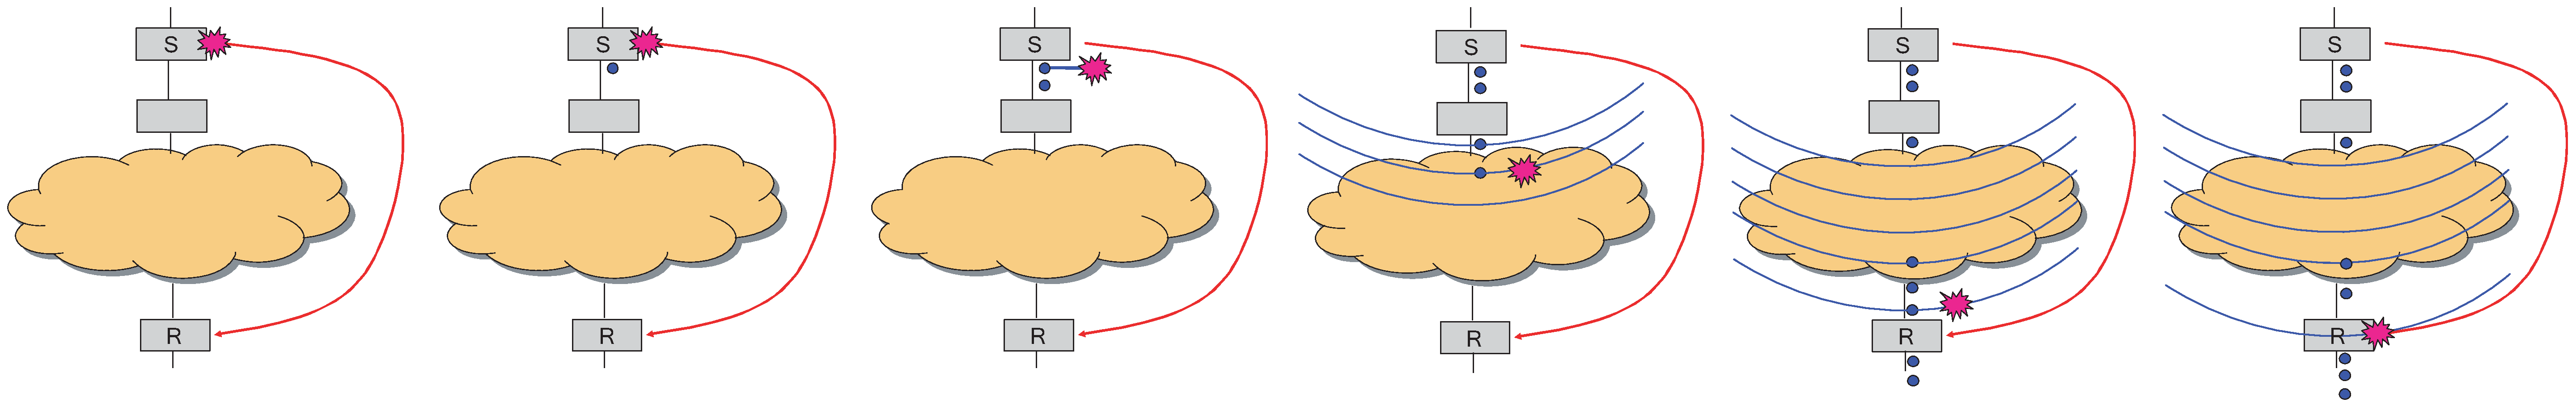
\includegraphics[width=6.5in]{thies1-1.eps}
    %    \vspace{1.05in}
  \end{center}
  \vspace{-30pt}
  \caption{Semantics of teleport messaging from $S$ to $R$ with
  latency one.  $S$ fires once and then (conceptually) tags its next
  output with the message.  The message propagates through the stream
  and is delivered when $R$ first sees the effects of the tagged
  item.}

  \vspace{-12pt}
\end{figure}

\absection{Progress}

We have completed a fully-automatic implementation of teleport
messaging in the StreamIt compiler, with a backend that targets a
cluster of workstations.  The output of the compiler is a set of
threads, each of which implements a component of the stream graph and
is allocated to a machine in a networked computing cluster.
Persistent, point-to-point TCP/IP channels are used for communication
between machines.  The message timing constraints are implemented with
a credit/acknowledegment system which maintains a loose
synchronization between each sender and receiver, thereby ensuring
that all messages sent can be received within the given time frame.

We have also performed a case study to evaluate the programmability
and performance implications of teleport messaging.  The application
of focus is a frequency hopping radio frontend, in which the receiver
switches between a set of known frequencies whenever it detects
certain tones from the transmitter.  A frequency change is indicated
by an up-stream message with a tight latency.  For comparison, we also
implemented a version that uses a feedback loop instead of messaging.

Using the StreamIt compiler to target a cluster of 16 Pentium~III
workstations, we obtain the following results.  The use of teleport
messaging reduces the volume of communicated data items by 35\%, and
results in a 50\% overall speedup.  In addition, teleport messaging
decreases the number of lines of code by 35\%, as it avoids the manual
implementation of timing constraints via the feedback loop.

\absection{Future}

There are three directions that we hope to explore in future work.
First, we need to implement a set of benchmarks that utilizes teleport
messaging and to expand our evaluation of the system with our current
backend.  Second, we plan to continue ongoing research that considers
the scheduling constraints implied by messages for a uniprocessor
backend such as a DSP~\cite{karczma-thesis}.  Finally, we aim to use
messaging as a starting point for developing more powerful dynamic
features, including morphing and re-initialization for sections of the
stream graph.  We believe that messaging could provide a good
mechanism for filters to trigger a wide range of dynamic adjustments
in adaptive stream programs.

%% This section is the one of the most important ones.  Please check 
%% with your research supervisor to make sure all the relevant funding
%% agencies for your project are acknowledged.

\absection{Research Support}
This work is supported in part by a grant from DARPA (PCA
F29601-04-2-0166), awards from NSF (CISE EIA-0071841, ITR ACI-0325297,
NGS CNS-0305453), and the MIT-Oxygen Project.

%% The abstract bibliographies should be done using bibtex.  Please
%% compile your bibtex entries into a single file with a distinguishing
%% name. The \absbibliography command is analogous to the \bibliography
%% command, taking a single argument, the name of your bibtex file, 
%% minus the .bib extention. The \bibliographystyle command should not
%% be used.  You can use a single bibliography file if you are submitting
%% multiple abstracts.  

\absbibliography{thies1}

\end{document}
